%%%%%%%%%%%%%%%%%%%%%%%%%%%%
% IEEE Consumer Electronics Magazine manuscript prepared from bare_lsens.tex.
% The author and publication metadata below remain anonymous/placeholders.
%%%%%%%%%%%%%%%%%%%%%%%%%%%%

\documentclass{IEEEmce}

\usepackage[colorlinks=true,urlcolor=blue,linkcolor=red,citecolor=blue]{hyperref}
\usepackage{upmath}
\usepackage{textcomp}
\usepackage[noadjust]{cite}
\usepackage[T1]{fontenc}
\usepackage{xcolor}
\usepackage{amsmath}
\interdisplaylinepenalty=2500
\usepackage[cmintegrals]{newtxmath}
\usepackage{bm}
\usepackage{array}
\usepackage{url}
\usepackage{graphicx}
\graphicspath{{./}{paper_assets/}}
\usepackage{tikz}
\usetikzlibrary{arrows.meta, positioning, calc}

\jvol{}
\jnum{}
\paper{}
\jmonth{Review draft}
\publisheddate{}
\currentdate{}
\jname{IEEE Consumer Electronics Magazine}
\pubyear{}
\doiinfo{}

\newtheorem{theorem}{Theorem}
\newtheorem{lemma}{Lemma}
\setcounter{secnumdepth}{0}

\renewcommand{\topfraction}{0.9}
\renewcommand{\bottomfraction}{0.8}
\renewcommand{\textfraction}{0.07}
\renewcommand{\floatpagefraction}{0.75}
\setcounter{topnumber}{3}
\setcounter{totalnumber}{4}

\hyphenation{op-tical net-works semi-conduc-tor}

% First-page footer identifies this working copy rather than a published article.
\makeatletter
\def\ps@plain{\let\@evenhead\@empty\let\@oddhead\@empty
\def\@oddfoot{\vbox{\hsize437pt{\rfxfont\bfseries Review draft}\hfill
\rlap{\hspace*{.75pc}\FolioODD}}}\let\@evenfoot\@oddfoot}
\makeatother
\begin{document}

\sptitle{Eye Blink Detection on Edge Hardware}

\title{Compact Embeddings\\
for Eye Blink Detection\\
on Edge Hardware}

\author{Hanul Yum}
\affil{Soonchunhyang University}

\author{Woojae Kim}
\affil{Institute for Molecular Metabolism Innovation}

\author{Hoyeon Ahn}
\affil{Soonchunhyang University}

\markboth{Eye Blink Detection on Edge Hardware}{Eye Blink Detection Using Low-Dimensional Embeddings for Real-Time Edge Deployment}

\begin{abstract}Camera-based eye blink monitoring is often deployed on edge-class hardware, where the
cost of the visual pipeline matters as much as its accuracy. We detect blink events on a
low-dimensional representation: each frame is encoded once into a 16-dimensional
embedding by a compact convolutional encoder, and a
temporal head classifies a buffer of these embeddings,
costing 0.37\% of the per-frame compute. On a 57-subject subset of the mEBAL2 database
(27{,}758 events, subject-disjoint five-fold cross-validation, three seeds), the
proposed model reaches a precision--recall AUC (PR-AUC) of $0.9886 \pm 0.0038$ against
$0.9906 \pm 0.0037$ for an image-based convolutional baseline with the same temporal
head. The paired subject-clustered difference, $-0.0040$ (95\% CI $[-0.0063,-0.0020]$),
lies within a non-inferiority margin of $\delta = 0.02$ fixed in advance, at $5.7\times$
fewer parameters and $2.6\times$ fewer multiply--accumulate operations. On a Raspberry
Pi~5 the representation stage costs $0.86$ against $2.05$~ms per frame, yet end to end
the control is only 11\% slower ($12.51$ against $11.27$~ms median), since landmark
detection dominates the pipeline.
\end{abstract}

% Keywords retained from the source manuscript: eye blink detection, learned
% representation, embedding, temporal convolutional network, edge computing,
% on-device inference.

\maketitle
\enlargethispage{10pt}

% =====================================================================
\chapterinitial{Spontaneous eye blinking} is a low-cost behavioral signal used for ocular surface stress
and attention estimation \cite{rosenfield2011,daza2020}. The practical question is not
whether blinks can be detected, but at what cost they can be detected continuously on
the device that holds the camera.

Two families of methods are widely used. Landmark-based methods reduce each frame to a
geometric ratio such as the eye aspect ratio (EAR) \cite{soukupova2016}, which is
negligible in cost once landmarks are available but compresses the eye region to a
single scalar. Image-based convolutional methods classify the eye crop directly
\cite{daza2020,daza2024}, retaining appearance information that a scalar discards, but
pay a convolutional cost over the full crop at every frame. Since the original EAR
formulation is itself a learned classifier over a temporal window of EAR values
\cite{soukupova2016}, we report both EAR variants to avoid understating that family.

We take an intermediate position (Figure~\ref{fig_pipeline}): each frame is encoded once
into an embedding $z \in \mathbb{R}^{16}$, buffered over the last 19 frames, and a
temporal convolutional head classifies the window on embeddings, so re-encoding is never
required.

Under a common crop, subject split and temporal head, we quantify the accuracy--cost
trade-off between a compact encoder and an adapted image-CNN reference. Both learned
frontends produce 16-dimensional features and both cache one representation per frame;
the controlled comparison is therefore between backbones. Our contributions are the
paired subject-level analysis of this trade-off, a transparent accounting of model and
pipeline cost, and a Raspberry Pi~5 stage decomposition showing that landmark detection
limits the end-to-end benefit. The stride and embedding-width ablations are exploratory
checks, not evidence of a uniquely optimal architecture.

% =====================================================================
\section{RELATED WORK}

Blink detection has used landmark ratios and learned temporal windows
\cite{soukupova2016}, per-frame convolutional classifiers with score aggregation
\cite{daza2020}, sequence models such as recurrent and transformer architectures
\cite{daza2024,fodor2023}, and dedicated in-the-wild benchmarks \cite{hu2019,zeng2023},
whose multi-person, untrimmed setting lies outside our single-user, event-level,
edge-CPU scope. Embedded blink detection has also reached wearable hardware
\cite{arcaya2021} and capacitive sensing \cite{capacitive2024}, both of which differ
from ours in sensing modality; closer to our approach, a 3-D autoencoder classifies
blinks from a learned latent code \cite{nousias2025}, but for offline video analysis,
aggregating per-frame predictions rather than one label per window, so it is not
included as a baseline. We instead target a representation compact enough to measure its
per-frame cost on an edge CPU.


\section{METHOD}
\begin{figure}[!t]
\centering
\resizebox{\columnwidth}{!}{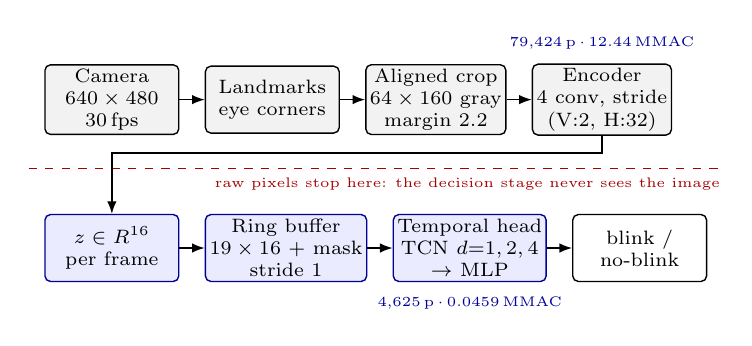
\begin{tikzpicture}[
font=\scriptsize,
  box/.style  = {draw, rounded corners=2pt, minimum height=8.5mm,
minimum width=17mm, align=center, inner sep=1.5pt, line width=0.5pt},
  pix/.style  = {box, fill=black!5},
  vec/.style  = {box, fill=blue!8, draw=blue!60!black},
  ar/.style   = {-{Latex[length=1.6mm]}, line width=0.5pt},
  cost/.style = {font=\tiny, text=blue!60!black},
  node distance = 3.2mm
]
\node[pix] (cam)  {Camera\\$640\times480$\\30\,fps};
\node[pix, right=of cam]  (mesh) {Landmarks\\eye corners};
\node[pix, right=of mesh] (crop) {Aligned crop\\$64\times160$ gray\\margin $2.2$};
\node[pix, right=of crop] (enc)  {Encoder\\4 conv, stride\\(V:2, H:32)};
\node[cost, above=0.6mm of enc] {79{,}424\,p\,$\cdot$\,12.44\,MMAC};
\draw[ar] (cam) -- (mesh);   \draw[ar] (mesh) -- (crop);   \draw[ar] (crop) -- (enc);
\node[vec, below=10mm of cam] (z)   {$z\in\mathbb{R}^{16}$\\per frame};
\node[vec, right=of z]        (ring){Ring buffer\\$19\times16$ + mask\\stride 1};
\node[vec, right=of ring]     (head){Temporal head\\TCN $d{=}1,2,4$\\$\rightarrow$ MLP};
\node[cost, below=0.6mm of head] {4{,}625\,p\,$\cdot$\,0.0459\,MMAC};
\node[box, right=of head] (out) {blink /\\no-blink};
\draw[ar] (z) -- (ring);   \draw[ar] (ring) -- (head);   \draw[ar] (head) -- (out);
\path (enc.south) -- (head.north) coordinate[pos=0.42] (mid);
\draw[red!65!black, dashed, line width=0.6pt]
($(cam.west |- mid)+(-2mm,0)$) -- ($(out.east |- mid)+(2mm,0)$);
\node[font=\tiny, text=red!65!black, fill=white, inner sep=1pt, anchor=north east]
at ($(out.east |- mid)+(2mm,-0.8mm)$)
{raw pixels stop here: the decision stage never sees the image};
\draw[ar] (enc.south) -- ++(0,-2.2mm) -| (z.north);
\end{tikzpicture}}
\caption{Proposed pipeline. Each frame is encoded once into a 16-dimensional embedding;
the 19-frame window is assembled from buffered vectors rather than re-encoded, so the
temporal head costs 0.37\% of the per-frame compute.}
\label{fig_pipeline}
\end{figure}

\subsection{Overview}
Figure~\ref{fig_pipeline} shows the pipeline: a rotation-aligned crop is encoded to
$z\in\mathbb{R}^{16}$, the last 19 embeddings are buffered, and a temporal convolutional
head with a small multilayer perceptron (MLP) emits a blink score. Landmark coordinates
are used only for the crop geometry and then discarded. The temporal head follows
standard dilated 1-D convolutions. The same buffering strategy applies to the image-CNN
reference; we measure the cost saved by replacing its backbone.

\subsection{Eye Crop Normalization}
Let $\bm p_L,\bm p_R\in\mathbb R^2$ be the landmark-derived eye centers (the midpoints
of the eye corners), $d_{\mathrm{io}}=\lVert\bm p_R-\bm p_L\rVert_2$, and $\bm c=(\bm
p_L+\bm p_R)/2$. We center a crop at $\bm c$, rotate it so that the inter-ocular axis is
horizontal, set its width to $w=2.2d_{\mathrm{io}}$, and resample it to a $H\times
W=64\times160$ grayscale image. Thus its source-image height is
$h_{\mathrm{crop}}=(H/W)w=0.88d_{\mathrm{io}}$; the scale is therefore normalized
against camera distance. Pixel values are standardized using only the current frame,
\begin{equation}
\tilde{x}_t=\frac{x_t-\mu_t}{\max(\sigma_t,0.255)},
\label{eq:normalization}
\end{equation}
where $\mu_t$ and $\sigma_t$ are the crop mean and standard deviation. The $0.255$ floor
equals $10^{-3}\times255$ and prevents division by zero. Out-of-border regions are
reflection-padded; resampling uses cubic interpolation when upsampling and area
interpolation when downsampling.

\subsection{Encoder Design and Vertical-Resolution Ablation}
\label{sec_encoder}
The encoder has four
Conv--BatchNorm--ReLU blocks with channels $(16,32,48,64)$, kernels
$(3\times5,3\times3,3\times3,3\times3)$, and strides $(1,4),(2,2),(1,2),(1,2)$ in
(vertical, horizontal) order, with no bias term since each is followed by batch
normalization. Same padding gives total strides of $2$ vertically and $32$ horizontally,
hence a $32\times5$ map. Horizontal average pooling reduces this to a $64\times32$
feature, which a linear layer maps to $D=16$. The encoder contains 79,424 parameters and
costs 12.44~MMAC per frame, 12.41 of it convolutional.

A matched \emph{v-drop} (reduced vertical resolution) variant keeps the kernels,
channels and horizontal strides unchanged while raising the vertical stride from $2$ to
$16$, cutting the convolutional cost from 12.41 to 3.44~MMAC; it is evaluated as an
exploratory ablation under \emph{Detection Accuracy}.

\subsection{Temporal Modeling on Embeddings}
\label{sec_temporal}
Re-encoding all $T=19$ frames at every decision would multiply the encoder cost by 19.
Instead, each frame is encoded once and the window is assembled from buffered vectors,
\begin{equation}
\bm z_t=f_\theta(\tilde{x}_t)\in\mathbb R^D,\qquad
\bm Z_t=[\bm z_{t-T+1}^{\mathsf T};\ldots;\bm z_t^{\mathsf T}]
\in\mathbb R^{T\times D}.
\label{eq:buffer}
\end{equation}
For every retained training/test event, $m_j\in\{0,1\}$ records whether window position
$j$ is valid, with $\sum_jm_j\ge14$. This is a dataset inclusion rule; a deployment
system must implement its own explicit missing-frame policy. The head uses
three residual 1-D Conv--BatchNorm--ReLU layers with kernel size 3 and dilations
$d_\ell\in\{1,2,4\}$:
\begin{equation}
\begin{aligned}
\bm s_j^{(\ell)}
&=\sum_{q=-1}^{1}\bm W_q^{(\ell)}
 [m_{j-d_\ell q}\bm h_{j-d_\ell q}^{(\ell-1)}],\\
\bm h_j^{(\ell)}
&=\operatorname{ReLU}\!\left(
\operatorname{BN}_\ell\!\left(\bm s_j^{(\ell)}+\bm b^{(\ell)}\right)\right)
+\bm h_j^{(\ell-1)},
\end{aligned}
\label{eq:tcn}
\end{equation}
where $\bm s_j^{(\ell)}$ is the masked convolutional sum,
$\bm h_j^{(0)}=\bm z_j$, and out-of-window indices are zero-padded, the default of
the 1-D convolution. The mask is applied to the buffer, before each convolution, and to
the final layer output; masked positions are excluded from both pooling operations,
\begin{equation}
\bm h_{\mathrm{avg}}=\frac{\sum_jm_j\bm h_j^{(3)}}{\max(1,\sum_jm_j)},
\qquad
\bm h_{\mathrm{max}}=\max_{j:m_j=1}\bm h_j^{(3)},
\label{eq:pooling}
\end{equation}
\begin{equation}
p=\varsigma\!\left(\operatorname{MLP}
([\,\bm h_{\mathrm{avg}};\bm h_{\mathrm{max}}\,])\right),
\label{eq:readout}
\end{equation}
where $\varsigma$ is the logistic function. The MLP has a 32-dimensional input, a
64-unit ReLU layer with dropout 0.3, and one logit output. Masking is not renormalized
by the number of valid taps, and symmetric padding lets a position use later frames
within its already collected window; the deployed decision requires no frames beyond the
current buffer, though a centered window places its center nine frames ($0.3$~s at 30~fps) before the decision.
This nominal alignment offset is not a measured onset-to-alert latency. The head costs 0.0459~MMAC per stride-1 decision, 0.37\% of the
12.49~MMAC per-frame model total.

\subsection{Reference Formulation}
For the EAR-rule baseline, $\mathrm{EAR}_j$ is the mean EAR of both eyes at valid
position $j$, and $j_f,j_l$ the first and last valid positions in the window. We use the
relative drop
$r_t=1-\min_{j:m_j=1}\mathrm{EAR}_j\,/\,[(\mathrm{EAR}_{j_f}+\mathrm{EAR}_{j_l})/2]$ and
select its classification threshold on the validation fold.

\section{EXPERIMENT}

\subsection{Dataset}
We use the RGB webcam stream of a 58-subject subset of the mEBAL2 database
\cite{daza2024}, whose full release contains 180 subjects and near-infrared channels we
do not use. The subset combines 38 subjects from the 2020 acquisition and 20 added in
2022. One subject (U18) is excluded (post hoc, not preregistered) because that session
was recorded with several people in frame and, whenever the primary subject was not
resolved, a neighboring person was cropped instead, affecting 31\% of that subject's
events. The remaining 57 subjects yield 27{,}758 events (13{,}820 blink, 13{,}938
no-blink). Each event is a fixed 19-frame window, and events with more than five
unresolved frames are excluded. The extraction stage stores 532{,}109 unique
$(\text{subject},\text{frame})$ crops --- a pipeline total covering the excluded
subject, later-discarded events, and crop reuse across overlapping events, not the
product of the event and window counts.

\subsection{Protocol}
We use subject-disjoint five-fold cross-validation, stratified jointly by event count
and acquisition batch, with three training seeds (15 runs). For rotation $i$, fold $i$
is the test fold, fold $(i+1)\bmod 5$ the validation fold, and the rest are used for
training. A threshold is selected only on the validation fold, maximizing accuracy over
all unique score values and their midpoints, then applied unchanged to the test fold.
All methods share the folds, seeds, threshold-selection code, and bootstrap
implementation, though the numeric grid is derived from each model's own validation
scores. The EAR rule is deterministic within a fold; EAR + head is a learned,
seed-dependent model.

\subsection{Training}
All learned methods use binary cross-entropy with logits, Adam (learning rate
$10^{-3}$), batch size 32, up to 80 epochs with early stopping (patience 10 on
validation PR-AUC), no data augmentation, and seeds $0,1,2$ with deterministic settings
enabled. The Image-CNN control is adapted from the mEBAL architecture \cite{daza2020} to
our $64\times160$ grayscale two-eye crop and event labels (adaptation details under
\emph{Baselines}).

\subsection{Baselines}
\label{sec_baselines}
Seven methods are compared. \emph{EAR (rule)} thresholds the relative EAR drop within
the window. \emph{EAR + head} lifts four per-frame features (left/right EAR, their mean
and minimum) to 16 channels via a $4\to16\to16$ BN+ReLU projection and feeds the same
temporal head. \emph{Image-CNN (max)} is the convolutional detector proposed by the
database authors \cite{daza2020}, with sequence scoring by the maximum of per-frame
scores as in the original. \emph{Image-CNN (+head)} replaces that aggregation with our
temporal head, leaving only the frontend different. \emph{Image-CNN (+BiLSTM)} and
\emph{Image-CNN (+LSTM)} keep the same Image-CNN backbone and swap in a single-layer
recurrent head of hidden size 16 (matched to the temporal convolutional network (TCN)
head) feeding the same MLP readout. BiLSTM runs forward and backward passes over the
window. Both recurrent heads use masked mean and max pooling over all recurrent outputs,
followed by an MLP; neither uses only the final hidden state. They see only the completed
buffer, although BiLSTM uses both directions within it. The 16-D Image-CNN backbone has
471,536 parameters, and the added TCN, BiLSTM and LSTM heads have 4,625, 8,577 and 4,353
parameters, respectively. The max variant has a 470,561-parameter scalar-output backbone;
its smaller projection must not be counted as a difference in temporal-head size.
\emph{Ours} uses the same 4,625-parameter TCN as Image-CNN (+head).

The recurrent accuracy rows were imported from a training handoff summary. Their raw
per-run predictions and trained checkpoints were not available for this revision;
we retain these rows as reported secondary results, not independently reanalysed evidence.


EAR is computed from the database's landmarks, so all methods share one detector and
face-selection rule; we use the stronger relative-drop EAR variant (PR-AUC $0.17$ higher
than a minimum-EAR rule, which is not reported separately). The image-based backbone is
not our design --- it is the architecture the database authors proposed and benchmarked
\cite{daza2020}, reducing the concern that we chose a weak baseline --- though it was
originally trained with per-frame open/closed labels rather than our
one-label-per-window protocol, so the max-pooling variant (trained under
multiple-instance supervision) may underestimate the original method.

\subsection{Metrics}
The primary metric is PR-AUC, with blink as the positive class; ROC-AUC, accuracy,
precision, recall, and $F_1$ are reported alongside. For each paired comparison we pool
the held-out predictions of all 15 runs, compute one PR-AUC difference, and resample the
57 subjects with replacement 2,000 times (each draw carries that subject's three seeds),
reporting percentile rather than bias-corrected 95\% intervals. For a reference method,
$\Delta=\mathrm{PR\mbox{-}AUC}_{\mathrm{ours}}- \mathrm{PR\mbox{-}AUC}_{\mathrm{ref}}$
is non-inferior when the lower limit of its paired 95\% confidence interval exceeds
$-\delta$, with $\delta=0.02$ specified before the final comparisons.

Cost covers parameters, MMAC per frame, latency percentiles, peak memory, CPU
utilization, idle-subtracted rail power and total-active rail energy per frame; operation counts include
only convolutions and linear projections (excluding bias, batch norm, activations,
pooling). One MAC is one multiply plus one add (two FLOPs); MMAC ($10^6$ MACs) is used
throughout so encoder, head and edge-measurement costs are directly comparable.

\subsection{Edge Platform}
Measurements use a Raspberry Pi~5 (16~GB, active cooling), Debian~13, Python~3.11, and
ONNX Runtime restricted to two intra-op threads with spinning disabled. The latency
frontend uses MediaPipe FaceMesh with one face and \texttt{refine\_landmarks=False}; the
accuracy experiments use the meshes distributed with mEBAL2. With the CPU governor set
to \texttt{performance}, six modes were replayed without frame-rate pacing, three times
each. Although the runner requested 300~s, the 18 power runs ended at the video boundary
after 98.65--130.39~s and 10,268 frames, achieving 78.75--104.09~fps. Thus these runs
characterize saturated offline throughput, not power at a matched 30~fps camera rate.
The configured PMIC sampling rate was 7.5~Hz; observed sampling was approximately
6.3~Hz after command overhead. The sum of 12 reported rails is provisional: the rail
definition was not independently verified and is not a whole-board input-power measure.
We report mean active-minus-idle power (30~s idle baseline), but energy per frame is
the trapezoidal integral of total active rail power divided by processed frames.
The two quantities must not be interpreted as the same idle-subtracted metric.
No throttling flags were reported in these runs. Separate earlier 300~s latency runs
provide the end-to-end medians quoted below; they are not the 18 power runs.


\begin{table*}[!t]
\caption{Blink Detection Performance and Static Cost. Subject-disjoint 5-fold $\times$ 3
seeds; 57 subjects, 27{,}758 events. PR-AUC and ROC-AUC are mean $\pm$ SD over 15 runs;
other metrics are 15-run means. Recurrent accuracy rows are imported summary values
whose raw prediction files were unavailable for this revision. MMAC counts operations after the landmark frontend,
profiled separately in Table~\ref{table_edge}. Red: best; bold: second-best, among the
image-based models (Image-CNN variants and Ours). EAR rows are landmark-only references
excluded from this ranking; the EAR rule's ``$\sim$0'' denotes a few divisions on six
landmark points, not a free method.}
\label{table_main}
\centering
\normalsize
\renewcommand{\arraystretch}{0.9}
\setlength{\tabcolsep}{2pt}
\begin{tabular*}{\textwidth}{@{}l@{\extracolsep{\fill}}cccccccc@{}}
\hline\hline
Method & PR-AUC $\uparrow$ & ROC-AUC $\uparrow$ & Acc $\uparrow$ & Prec $\uparrow$ & Rec $\uparrow$ & F1 $\uparrow$ & MMAC $\downarrow$ & Params $\downarrow$\\
\hline
EAR (rule)              & 0.8931 $\pm$ 0.0136 & 0.9169 $\pm$ 0.0146 & 0.8505 & 0.8268 & 0.8878 & 0.8550 & $\sim$0 & 0\\
EAR + head              & 0.9724 $\pm$ 0.0096 & 0.9738 $\pm$ 0.0113 & 0.9276 & 0.9312 & 0.9228 & 0.9268 & 0.05 & 5{,}009\\
Image-CNN (max) \cite{daza2020} & 0.9114 $\pm$ 0.0291 & 0.9404 $\pm$ 0.0207 & 0.8917 & 0.8526 & 0.9480 & 0.8971 & \textbf{31.81} & \textbf{470{,}561}\\
Image-CNN (+head) & \textcolor{red}{0.9906 $\pm$ 0.0037} & \textcolor{red}{0.9930 $\pm$ 0.0036} & \textcolor{red}{0.9651} & \textcolor{red}{0.9713} & 0.9584 & \textcolor{red}{0.9644} & 31.85 & 476{,}161\\
Image-CNN (+BiLSTM)     & 0.9850 $\pm$ 0.0060 & 0.9889 $\pm$ 0.0048 & 0.9542 & 0.9559 & 0.9524 & 0.9536 & 31.89 & 480{,}113\\
Image-CNN (+LSTM)       & 0.9819 $\pm$ 0.0199 & 0.9891 $\pm$ 0.0069 & 0.9615 & 0.9571 & \textcolor{red}{0.9665} & 0.9615 & 31.85 & 475{,}889\\
Ours ($D=16$)  & \textbf{0.9886 $\pm$ 0.0038} & \textbf{0.9914 $\pm$ 0.0037} & \textbf{0.9620} & \textbf{0.9605} & \textbf{0.9636} & \textbf{0.9618} & \textcolor{red}{12.49} & \textcolor{red}{84{,}049}\\
\hline\hline
\end{tabular*}
\end{table*}

\subsection{Detection Accuracy}
\label{sec_accuracy}
Table~\ref{table_main} reports the runs. The best PR-AUC in the table is not ours: the
image-based backbone with our temporal head reaches $0.9906 \pm 0.0037$ against our
$0.9886 \pm 0.0038$. Our claim is about cost, not accuracy. The paired subject-clustered
difference between the two is $-0.0040$ with a 95\% CI of $[-0.0063,-0.0020]$. That
interval excludes zero, so the proposed model is measurably the less accurate of the
two, but lies inside the prespecified margin $\delta = 0.02$; on the same folds it uses
$5.7\times$ fewer parameters ($84{,}049$ against $476{,}161$) and $2.6\times$ fewer
operations per frame.

The mean of the 15 paired run differences is $-0.0019\pm0.0024$. Pooling scores from
different fitted models and averaging their AP values are different estimands; their
values must not be interchanged. In a post-hoc margin sensitivity analysis, the primary
pooled interval also supports $\delta=0.01$, but not $\delta=0.005$. The original
$0.02$ margin was informed by reference variability, not independently validated as a
clinically or operationally acceptable loss.

A second post-hoc analysis gives each subject equal weight: average that subject's AP
over its three source runs, then average the 57 subjects. The paired difference is
$-0.0062$ (subject bootstrap 95\% CI $[-0.0114,-0.0023]$). This supports $0.02$ but
not $0.01$, showing that the stronger margin conclusion depends on weighting.
These intervals condition on the saved fits and do not capture full retraining uncertainty.

The recurrent summary rows suggest sensitivity to head choice, but do not support
new paired inference without their raw predictions. A confidence interval excluding
zero cannot be dismissed merely because its effect is smaller than a seed standard
deviation. The Image-CNN backbone accounts for essentially all of the recurrent
variants' static computational cost. Its 6,912-to-64 dense layer alone has 442,432
parameters; the reported parameter ratio is therefore specific to this adapted
reference and does not establish superiority over all lightweight CNNs.


The exploratory \emph{v-drop} ablation described under \emph{Encoder Design and
Vertical-Resolution Ablation} gives a paired
PR-AUC estimate of $+0.0010$ for the proposed encoder (95\% CI $[-0.0032,+0.0069]$)
across folds 0--1 and three seeds (21 subjects); covering only two of five folds, this
is descriptive rather than evidence that vertical resolution is irrelevant, and we
retain the proposed encoder.

\subsection{Robustness across Conditions}
Against EAR + head, the pooled-prediction advantage is $+0.0151$ overall. The exploratory
analyses include acquisition batch (two groups), glasses (two groups), and brightness,
contrast and sharpness terciles (nine groups). Their unadjusted intervals describe
observed heterogeneity; they are not simultaneous guarantees of robustness. Against
Image-CNN (+head), the available paired subgroup analysis covers acquisition batch and
glasses, plus the overall result. Those intervals meet $\delta=0.02$; corresponding
photometric comparisons were not available. Natural subgroup differences do not replace
controlled tests of illumination, pose or viewing distance.


\subsection{Model Complexity and Edge Performance}
\label{sec_edge}

\begin{table}[!t]
\caption{Per-Frame Latency and Power/Energy Cost on a Raspberry Pi~5, measured together
over three free-running repeats (98.65--130.39~s each). Latencies are ms/frame. Crop = eye-crop extraction; Enc. = encoder
forward pass; Dec. = decision stage; Sub. = sum of stage medians, not a measured subtotal percentile; e2e99 = 99th-percentile
end-to-end latency; $\Delta$P(W) = active-minus-idle rail power; mJ/frame = total-active
rail energy. Rail definition is unverified. Lower is better; bold
marks the best learned model in each column.}
\label{table_edge}
\centering
\normalsize
\renewcommand{\arraystretch}{0.9}
\setlength{\tabcolsep}{3pt}
\begin{tabular*}{\columnwidth}{@{}l@{\extracolsep{\fill}}cccc@{}}
\hline\hline
Method & Crop & Enc. & Dec. & Sub.\\
\hline
EAR (rule, ref.)    & 0.08 & ---  & 0.14 & 0.22\\
\textbf{Ours}       & 0.67 & \textbf{0.86} & 0.25 & \textbf{1.78}\\
Image-CNN (max)     & 0.67 & 2.04 & \textbf{0.17} & 2.88\\
Image-CNN (+head)   & 0.67 & 2.05 & 0.31 & 3.03\\
Image-CNN (+BiLSTM) & 0.67 & 2.05 & 0.36 & 3.08\\
Image-CNN (+LSTM)   & 0.67 & 2.04 & 0.33 & 3.03\\
\hline\hline
\end{tabular*}
\vspace{3pt}

\begin{tabular*}{\columnwidth}{@{}l@{\extracolsep{\fill}}ccc@{}}
\hline\hline
Method & e2e99 & $\Delta$P(W) & mJ/frame\\
\hline
EAR (rule, ref.)    & 10.21 & 2.155 & 40.70\\
\textbf{Ours}       & \textbf{11.88} & \textbf{2.000} & \textbf{46.15}\\
Image-CNN (max)     & 12.96 & 2.260 & 53.77\\
Image-CNN (+head)   & 13.17 & 2.209 & 53.88\\
Image-CNN (+BiLSTM) & 13.24 & 2.200 & 54.38\\
Image-CNN (+LSTM)   & 13.17 & 2.202 & 54.36\\
\hline\hline
\end{tabular*}
\end{table}

Frame read ($\sim$1~ms) and landmark detection (8.3--8.5~ms) are shared by all modes and
account for most of the crop-to-e2e gap; EAR (rule), having no encoder, is excluded from
the \emph{crop} comparison. The Image-CNN graphs were exported with random weights for
structural latency and power characterization, so these measurements do not demonstrate
the runtime/energy of the trained accuracy checkpoints in
Table~\ref{table_main}. At the representation stage the proposed encoder costs $0.86$~ms
per frame against $2.05$~ms for the Image-CNN (+head) control, a $2.4\times$ reduction,
close to the $2.6\times$ static ratio in multiply--accumulate operations; over the
method-specific stages together (crop, encode, decide) the ratio is $1.7\times$.

End to end, the proposed system has a median latency of $11.27$~ms and the control
$12.51$~ms, i.e. the control is 11\% slower. The shared landmark stage accounts for
66--75\% of these medians. The observed 99th percentiles are below the $33.3$~ms frame period, supporting
processing headroom on this replay. This does not establish live-camera deadline
reliability or a bound on onset-to-alert delay.

Under free-running replay, the proposed model draws $2.000$~W above the measured idle
rail sum and uses $46.15$~mJ/frame of total active rail energy, versus
$53.77$--$54.38$~mJ/frame for the image-CNN variants. Different achieved frame rates,
short runs, unverified rails and random-weight comparison graphs prevent a claim of
energy savings at a matched 30~fps workload or an inferred battery lifetime.

The latency decomposition is the more direct system result. From the earlier mean
latencies, even eliminating the 0.868~ms encoder would reduce the 11.300~ms pipeline
by only 7.7\%, assuming all other stages stay fixed. Halving the 8.487~ms landmark stage
would instead save 37.6\% under that same assumption. These are arithmetic upper-bound
scenarios, not measured frontend optimizations.


\subsection{External Continuous-Video Pilot}
We additionally evaluate the locally available original EyeBlink8 video~9
\cite{fogelton2016,eyeblink8data}: one person, 41 annotated blink IDs. This is one of
eight benchmark videos and had previously been used without accuracy labels for timing.
The container and timestamp file list 5,183 frames, but 5,134 decode, and the annotation
ends at decoded frame 5,133 (zero-based). We discard the 49 unmatched tail timestamps.
Nearest-frame resampling using capture times gives 5,133 positions at 30~Hz, with 174
duplicates and 175 unused native frames. MediaPipe crop coverage is 99.75\%; all
annotated evaluation windows meet the 14-of-19 validity rule. Sampled annotation/eye-corner
alignment and checkpoint reproduction were checked as implementation audits.

All 15 source-trained checkpoints and their source-validation thresholds are frozen.
No external training, threshold selection or best-run selection is performed. The
window diagnostic uses 41 blink-centered windows and 210 deterministic, non-overlapping
negative windows without blink overlap. Continuous evaluation thresholds every trailing
window and groups consecutive positives, without tuned hysteresis. Predicted intervals
are aligned to the window center and matched one-to-one to overlapping blink-ID
intervals. All 41 blinks are included over 2.80 annotated minutes. This bilateral-ID
protocol is distinct from the dataset authors' per-eye completeness evaluation.

\begin{table}[!t]
\caption{Descriptive external pilot: one EyeBlink8 video. Means over 15 source fits;
these fits are not 15 independent external subjects. AP refers to sampled windows;
R, F1 and false events/minute (FA/min) refer to continuous detection.}
\label{table_external}
\centering\small\setlength{\tabcolsep}{3pt}
\begin{tabular*}{\columnwidth}{@{}l@{\extracolsep{\fill}}cccc@{}}
\hline
Method & AP & R & F1 & FA/min\\
\hline
Ours & 0.999 & 0.998 & 0.889 & 3.81 \\
Image-CNN (+head) & 0.999 & 0.992 & 0.867 & 4.93 \\
EAR + head & 0.965 & 1.000 & 0.691 & 13.28 \\
EAR (rule) & 0.998 & 1.000 & 0.875 & 4.21 \\
\hline
\end{tabular*}
\end{table}

The proposed model's continuous F1 varies from 0.726 to 0.976 across source fits
(mean 0.889, SD 0.063), despite a mean window AP of 0.999. It produces 3.81 unmatched
detections/minute on average (SD 2.57), and its negative-frame positive rate is 0.63\%.
Requiring temporal intersection-over-union of at least 0.1 gives the same proposed-model
F1 here. The mean of run-wise median onset-to-first-decision offsets is 0.307~s, computed
from capture timestamps and excluding processing, display and queue delays. This pilot
demonstrates a measurable classification-to-continuous-detection gap; its single subject
cannot establish cross-dataset superiority or a population confidence interval.

\subsection{Discussion and Limitations}
The failure on held-out subject U1 remains unresolved: its mean AP is $0.8200$ versus
$0.9433$ for Image-CNN (+head) and $0.9802$ for EAR + head. Existing diagnostic checks
do not establish a causal explanation or exclude all annotation/preprocessing effects.
U1 is retained in every primary analysis; removing it changes the pooled image-control
difference only from $-0.00402$ to $-0.00388$, so it does not explain the full trade-off.

The primary benchmark classifies fixed 19-frame events, not continuous detections.
Its balanced negative sampling and validation accuracy threshold do not determine the
false-alarm rate at deployment prevalence. The nominal 0.3~s center offset is separate
from compute latency and from measured alert delay. The primary width was fixed at
$D=16$ before final comparisons; exploratory $D=8,32,64$ results on two folds exist,
so the width was not wholly unswept. They do not establish a global optimum. The
vertical-stride ablation likewise does not support the proposed geometry as necessary.
The one-subject external pilot does not establish generalization beyond the
57-subject source subset; landmark-source shift is not resolved by using the
same crop code.


\section{CONCLUSION}
A compact encoder with a shared temporal head yields a measured accuracy--cost
trade-off on subject-disjoint mEBAL2 events: the pooled AP loss is small but nonzero,
and falls within the prespecified $0.02$ margin at $5.7\times$ fewer parameters and
$2.6\times$ fewer operations than the adapted Image-CNN control. Both frontends use
cached 16-D features. Raspberry Pi~5 replay shows ample compute headroom, while its
dominant landmark stage limits the benefit of encoder compression. Stronger deployment
claims require continuous external evaluation and matched-rate, verified power measurements.


\section{ACKNOWLEDGMENTS}
Hanul Yum is the corresponding author
(email: \href{mailto:hanoo11213@sch.ac.kr}{hanoo11213@sch.ac.kr}).

% Compact reference leading prevents a nearly empty final page; font size is unchanged.
\renewcommand{\bibliofont}{\fontfamily{\sfdefault}\fontsize{8}{11.5}\selectfont\raggedright}
\begin{thebibliography}{12}

\bibitem{rosenfield2011}
M.~Rosenfield, ``Computer vision syndrome: A review of ocular causes and potential
treatments,'' \emph{Ophthalmic Physiol. Opt.}, vol.~31, no.~5, pp.~502--515, 2011.

\bibitem{daza2020}
R.~Daza, A.~Morales, J.~Fierrez, and R.~Tolosana, ``mEBAL: A multimodal database for eye
blink detection and attention level estimation,'' in \emph{Proc. ACM Int. Conf.
Multimodal Interact. (ICMI) Companion}, 2020, pp.~32--36.

\bibitem{soukupova2016}
T.~Soukupov\'{a} and J.~\v{C}ech, ``Real-time eye blink detection using facial
landmarks,'' in \emph{Proc. Comput. Vis. Winter Workshop (CVWW)}, 2016.

\bibitem{daza2024}
R.~Daza, A.~Morales, J.~Fierrez, R.~Tolosana, and R.~Vera-Rodriguez, ``mEBAL2 database
and benchmark: Image-based multispectral eyeblink detection,'' \emph{Pattern Recognit.
Lett.}, vol.~182, pp.~83--89, 2024.

\bibitem{fodor2023}
\'{A}.~Fodor, K.~Fenech, and A.~L\H{o}rincz, ``BlinkLinMulT: Transformer-based eye blink
detection,'' \emph{J. Imaging}, vol.~9, no.~10, art.~196, 2023.

\bibitem{hu2019}
G.~Hu, Y.~Xiao, Z.~Cao, L.~Meng, Z.~Fang, J.~T. Zhou, and J.~Yuan, ``Towards real-time eyeblink
detection in the wild: Dataset, theory and practices,'' \emph{IEEE Trans. Inf. Forensics
Security}, vol.~15, pp.~2194--2208, 2020.

\bibitem{zeng2023}
W.~Zeng \textit{et al.}, ``Real-time multi-person eyeblink detection in the wild for
untrimmed video,'' in \emph{Proc. IEEE/CVF Conf. Comput. Vis. Pattern Recognit. (CVPR)},
2023, pp.~13854--13863.

\bibitem{arcaya2021}
A.~Arcaya~Jordan, A.~Pegatoquet, A.~Castagnetti, J.~Raybaut, and P.~Le~Coz, ``Deep
learning for eye blink detection implemented at the edge,'' \emph{IEEE Embed. Syst.
Lett.}, vol.~13, no.~3, pp.~130--133, 2021.

\bibitem{capacitive2024}
M.~Liu, S.~Bian, Z.~Zhao, B.~Zhou, and P.~Lukowicz, ``Energy-efficient, low-latency, and
non-contact eye blink detection with capacitive sensing,'' \emph{Front. Comput. Sci.},
vol.~6, art.~1394397, 2024.

\bibitem{nousias2025}
G.~Nousias, K.~K. Delibasis, and G.~Labiris, ``Blink detection using 3D convolutional
neural architectures and analysis of accumulated frame predictions,'' \emph{J. Imaging},
vol.~11, no.~1, art.~27, 2025.

\bibitem{fogelton2016}
A.~Fogelton and W.~Benesova, ``Eye blink detection based on motion vectors analysis,''
\emph{Comput. Vis. Image Underst.}, vol.~148, pp.~23--33, 2016.

\bibitem{eyeblink8data}
Blinking Matters, ``Research: EyeBlink8 dataset and annotations,'' accessed Sep.~18, 2026.
[Online]. Available: \url{https://www.blinkingmatters.com/research}

\end{thebibliography}

\end{document}
